

\section{Data and interaction}
The data recorded by multiple detectors are stored in different partitions. Before carrying out the stability test in this project, the data being analyzed are already pre-selected. In this section, an overview about data storage and pre-selection is discussed, followed by a short introduction of probable interaction giving rise to selected data.

\begin{figure}[t!]
	\centering
	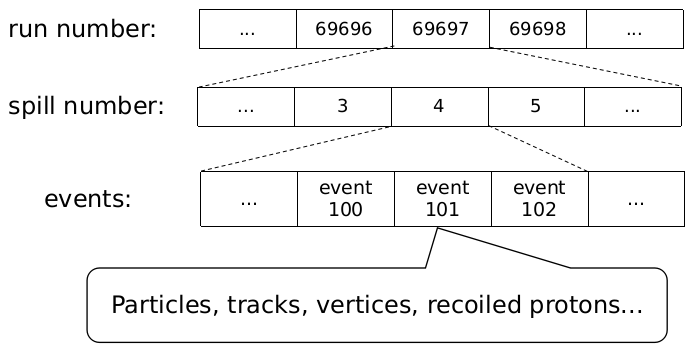
\includegraphics[width=0.5\textwidth]{data_storage}
	\caption{Scheme of data storage structure. Data from the detectors are categorized into three different levels.}
	\label{fig:data_storage}
\end{figure}

\subsection{Data storage}
There are three different partition levels regarding the data storage, as is shown in picture \ref{fig:data_storage}. First, the whole data are stored with different run number. The event data with same run number are further divided into different spill number. One spill corresponds to one period of process, in which the particle beam is bunched and de-bunched. Time expansion of each spill is around 48 seconds \cite{COMPASS}, which is time period of SPS (super proton synchrotron). Similarly, each spill contains large amount of events. One event represents a single scattering between $\pi$ and proton and it contains all data of the corresponding event from detectors such as tracking detectors or calorimeters.

\subsection{Data preselection}
\label{subsec:data_preselection}
The data used in this stability test are not raw data coming directly from detectors, but rather being preselected previously. Event is only selected if it meets following 4 conditions: 
\begin{itemize}
	\item A best primary vertex was found
	\item Primary vertex Z-position $Z_{pv}$: $\SI{-200}{\centi\meter} < Z_{pv} < \SI{160}{\centi\meter}$
	\item Exactly one or three charged tracks, leaving the primary vertex
	\item Charge sum of all three tracks $= -1$
\end{itemize}
The first condition requires the existence of primary vertex. This is because the vertex position is not the value that can be directly measured by detectors. It is rather reconstructed by identifying the intersecting point between two charged particle tracks. Thus, there could be no primary vertex constructed in some events, which should be selected out. Second condition excludes the events where outgoing particles are not coming from the interaction on proton target but rather on some detectors. Therefore, the position of primary vertex must be around the target region. The third and fourth condition guarantees the data after selection correspond to the elastic scattering or the interaction where one $\pi$ is scattered into three charged $\pi$.

\subsection{Scattering process}
\label{subsec:photon}
\begin{figure}[thb]
	\centering
	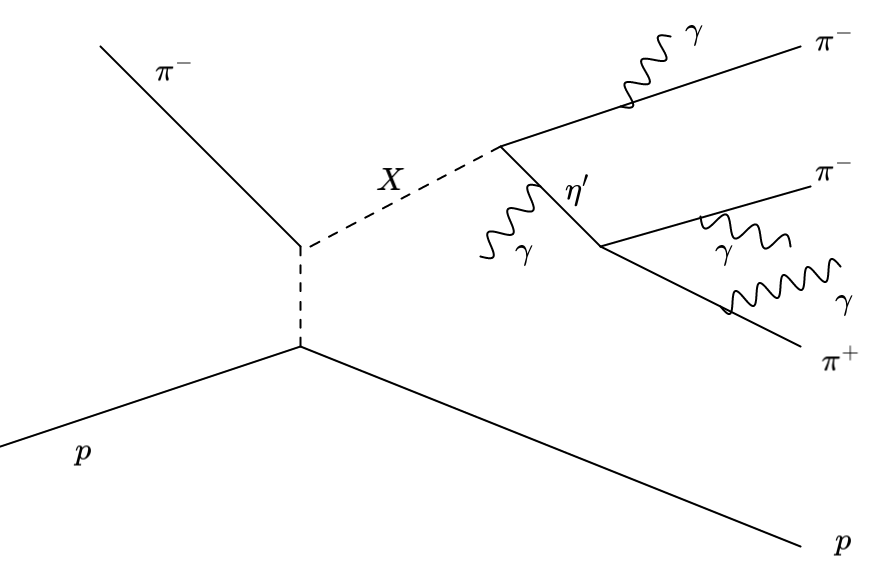
\includegraphics[width=0.5\textwidth]{feymann_diag}
	\caption{Scheme of one possible inelastic scattering between $\pi$ and proton. In such case, $pi^-$ is excited and consecutively decays into 3 charged $\pi$, during which multiple photons can also be emitted.}
	\label{fig:feymann_diag}
\end{figure}

The interaction that is looked into for this stability test is inelastic scattering of one $\pi^-$ scattered into three charged $\pi$. Due to the preselection, charged ejectile particles are very likely to be $\pi^-$, $\pi^+$, $\pi^-$.  One possibility of the interaction is shown in figure \ref{fig:feymann_diag}. By scattering off the proton target, $\pi^-$ is excited into a high energy state ($X$), which in a very short time, decays into $\pi^-$ and $\eta'$. Due to instability of $\eta'$, it finally decays into $\pi^-$ and $\pi^+$ as well. Meanwhile, certain number of photons can also be emitted by electromagnetic radiation. 